\documentclass[acmsmall]{acmart}

\setcopyright{rightsretained}
\copyrightyear{2021}
\acmYear{2021}
\acmConference[HATRA '21]{Human Aspects of Types and Reasoning Assistants}{October 2021}{Chicago, IL}

\begin{document}

\title{Position Paper: Goals of the Luau Type System}

\author{Andy Friesen}
\author{Alan Jeffrey}
\author{Other People?}
\affiliation{
  \institution{Roblox}
  \city{San Mateo}
  \state{CA}
  \country{USA}
}

\begin{abstract}
  A position paper about goals of the Luau type system.
\end{abstract}

\maketitle

\section{Introduction}

The Roblox~\cite{Roblox} platform allows anyone to create shared,
immersive, 3D experiences.  At the time of writing, there are
approximately eight million experiences available on Roblox, created
by eight million developers.  Roblox creators are often young, for
example there are over 200 Roblox kids' coding camps in over 65 countries
listed at~\cite{AllEducators}.

The Luau programming language~\cite{Luau} is the scripting language
used by developers of Roblox experiences. Luau is derived from the Lua
programming language~\cite{Lua}, with additional capabilities,
including a type inference engine.

This paper will discuss some of the goals of the Luau type system,
focusing on where the goals are different from those of other type systems.

\section{Human Aspects}
\subsection{Heterogenous developer community}

Quoting a 2020 report \cite{RobloxDevelopers}:
\begin{itemize}
\item Adopt Me! now has over 10 billion plays and surpassed 1.6 million concurrent users in game earlier this year.
\item Piggy, launched in January 2020, has close to 5 billion visits in just over six months.
\item There are now 345,000 developers on the platform who are monetizing their games.
\end{itemize}
This demonstrates how heterogenous the Roblox developer community is:
developers of experiences with plays measured in billions are on the same
platform as children first learning to code. Moreover, \emph{both of
these groups are important}, as the professional development studios
bring high-quality experiences to the platform, and the beginning creators
contribute to the energetic creative community.

\subsection{Goal-driven learning}

All developers are goal-driven, but this is especially true for
learners. A learner will download Roblox Studio (the IDE) with an
experience in mind, often designing an obstacle course (an ``obby'')
to play in with their friends.

The user experience of developing a Roblox experience is primarily a
3D interactive one, seen in Fig.~\ref{fig:studio}(a). The user designs
and deploys 3D assets such as terrain, parts and joints, and provides
them with physics attributes such as mass and orientation. The user
can interact with the experience in Studio, and deploy it to a Roblox
server so anyone with the Roblox app can play it.

\begin{figure}
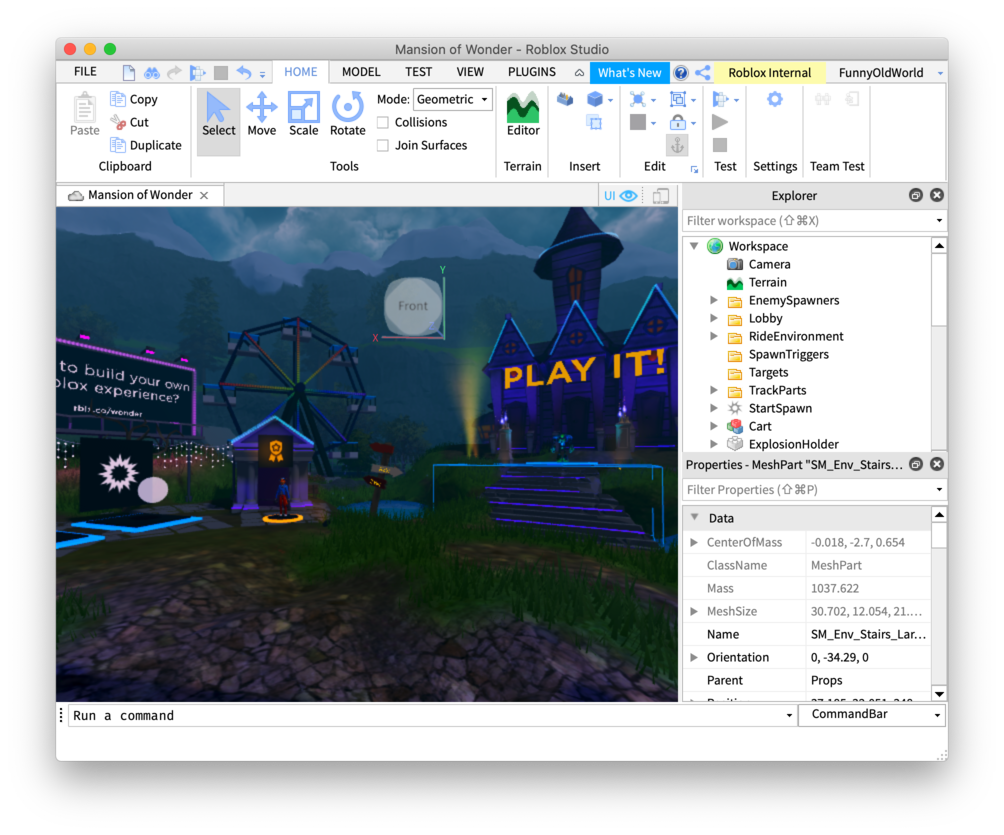
\includegraphics[width=0.48\textwidth]{studio-mow.png}
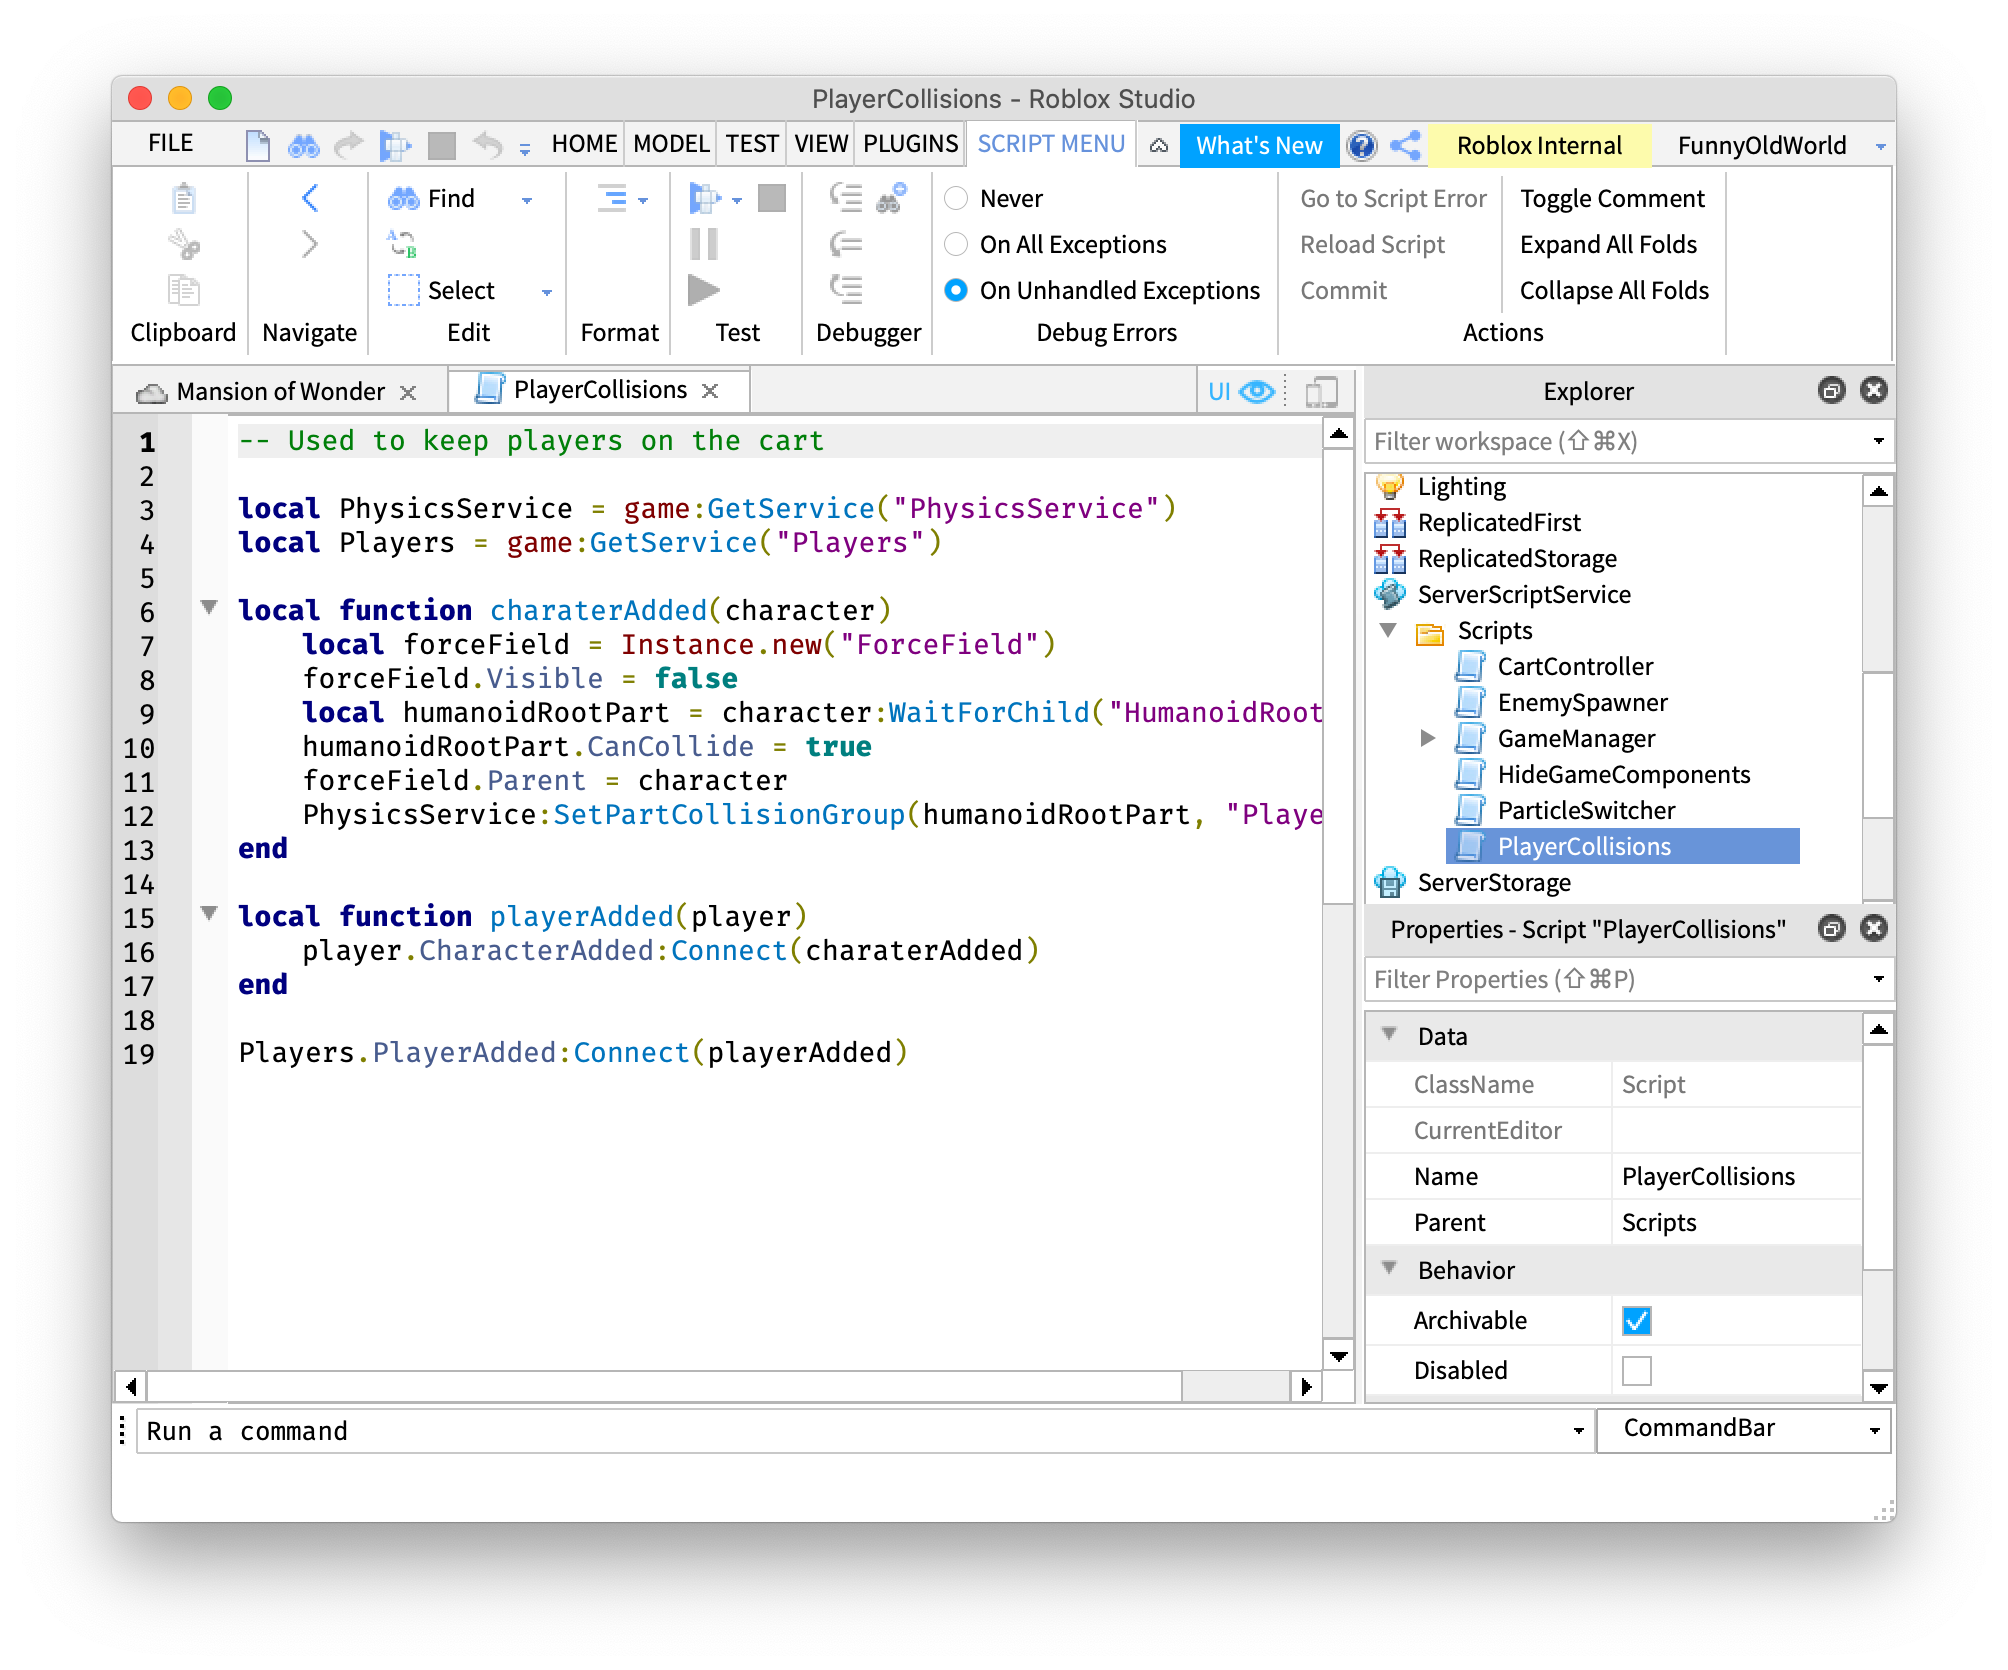
\includegraphics[width=0.48\textwidth]{studio-script-editor.png}
\caption{Roblox Studio's 3D environment editor (a), and script editor (b)}
\label{fig:studio}
\end{figure}

At some point during experience design, the user of Studio has a need
which can't be met by the physics engine alone. ``The stairs should
light up when a player walks on them'' or ``a firework is set off
every few seconds.'' At this point they will discover the script
editor, seen in Fig.~\ref{fig:studio}(b), and the Luau programming language.

This onboarding experience is different from many initial exposures to
programming, in that by the time the user first opens the script
editor, they have already built much of their creation, and have a
very specific concrete aim.  It suggests a Luau goal for helping the
majority of creators: \emph{support learning how to perform specific
tasks} (for example through autocomplete suggestions and
documentation).

\subsection{Type-driven development}

- Code refactoring

- Code navigation

- Detect detection

\section{Types}
\subsection{Infallible types}

Goal: support type-directed tools in all programs

- All programs have a type (analogy with infallible parsers)

- Used by autocomplete + goto-declaration

- Still support red squigglies

- Problem: stop the user being swamped by cascading errors

- Problem: no ``right'' type, just heuristics

\subsection{Strict types}

Goal: no false negatives

- Appropriate for experienced developers?

- Variants of ``usual techniques'' apply, e.g. progress becomes ``if you get stuck, there must be red squigglies''

- Related to blame analysis?

\subsection{Nonstrict types}

Goal: no false positives

- Appropriate for the majority of developers?

- Usual techniques do not apply, e.g. correctness becomes ``code with red squigglies does not return a result''

- Related to success types?

- Problems with mutation and avoiding whole-program analysis.

\subsection{Mixing types}

Goal: support mixed strict/nonstrict development

- Strictness is per-script, so programs are mixed

- Can the correctness criteria be combined?

- Can success types be combined with regular types?

- Same types, different red squigglies?

- Related: incorrectness logic vs correcness logic?

\section{Future work}

Draw the damn owl

- Mixing types

- Other interactions between types and IDEs, e.g. typed holes.

- Formalizations of all of this?

\bibliographystyle{ACM-Reference-Format} \bibliography{bibliography}

\end{document}
